%----------------------------------------
% Write your notes here
%----------------------------------------

\section{Learning by Example}

How did we (as humans) resolve spam vs. real emails when cleaning up an inbox?
\begin{itemize}
\item Key-word searches
\item Look for email contacts, but maybe there are necessary unknown contacts 
\item Use what is already in the inbox
\item Did the email go out to a large group of people, BUT lots of email lists are legit
\end{itemize}

We have a lot of options, but they are weakly indicative of what is or is not spam. How do we make a direct rule out of this? We could use a bunch of if-then statements, then that could get really complicated because each statement has to be weighted differently. This is the idea of building a \textbf{classifier}. We learn the rules from the data.

\section{Exercise: Diagnoses a la Bayes}

Suppose we are testing for a rare disease. $1$\% of the population is infected, and we have a highly sensitive and specific test that yields $99$\% of sick patients test positive, $99$\% of healthy patients test negative. Given a patient tests positive, what is the probability the patient is sick?

\graphicspath{Diagnoses}

\section{Natural frequencies a la Gigerenzer}

Claim: early screening of breast cancer lowers chance of breast cancer by 20\%. What does this mean? Imagine there are a thousand women who do not get screened and a thousand women who do get screened. $5$ women who did not get screening died of breast cancer. $4$ women who did get screening died of breast cancer, so we are comparing $\frac{5}{1000}$ and $\frac{4}{1000}$. Also note that the number of women who died from all types of cancer is equal ($21$ overall).

If a woman does not get screening, then there is no cost. If you do get screening there is a different cost (what if it is a false alarm?). After perhaps surgery a lot of women learned they didn't have breast cancer. If the test is not reliable enough, it can cause a lot of false positives and unnecessarily scare people. Note that the guidelines of early screening have changed. Genetic markers and other indicators means screening is recommended.

\section{Inverting conditional probabilities}

Let us start with the \textbf{product rule}

$$p(y | x) p(x) = p(x, y) ~~~~~~~~~~~~~~~ p(x | y) p(y) = p(x, y).$$

Equating both sides we get

$$p(y | x) p(x) = p(x, y) = p(x | y) p(y).$$

If we divide both sides by $p(x)$, we get

$$p(y | x) = \frac{p(x | y) p(y)}{p(x)},$$

which is \textbf{Bayes' Theorem}.

\textbf{Bayes' Theorem} states 

$$p(y | x) = \frac{p(x | y) p(y)}{p(x)},$$

where $p(x) = \sum_{y \in \Omega y} p(x | y) p(y)$ is the normalization constant. 

There is a truth and then there is an indicator (positive or negative)

\section{(Super) Naive Bayes}

In the email, we define 'truth' as whether or not an email is spam. We use indicators tell us which is which. Bayes' Rule allows us to do this. Using the branches from previously, we let $p(y)$ denote the 'positive' branches.

Going back to the suggestion of looking at different emails and see how often different words occur. Bayes' rule let's us do that. Look among all the emails that are spam and search for a key word. This is Super Native Bayes, where we classify the emails based on one word. We take all the spam documents containing the keyword and divide by all the spam docs. We need the probability of seeing the words among both spam and non-spam documents. Note, we call non-spam 'ham'. Let $h$ denote ham, $s$ denote spam, and $w$ denote all the words. So we have:

$$p(w) = p(w | s)p(s) + p(w |h)p(h)$$

Note: we care about how often does the word occurs overall, not just how many documents it appears in. Even though we only care about spam, we have to look in both spam and ham. We ask the question: what are the sizes of that term relative to the other sizes?

We can also use shell to do this by looking at released Enron employee emails to build our script, which does everything from get the data to build the classifier. 

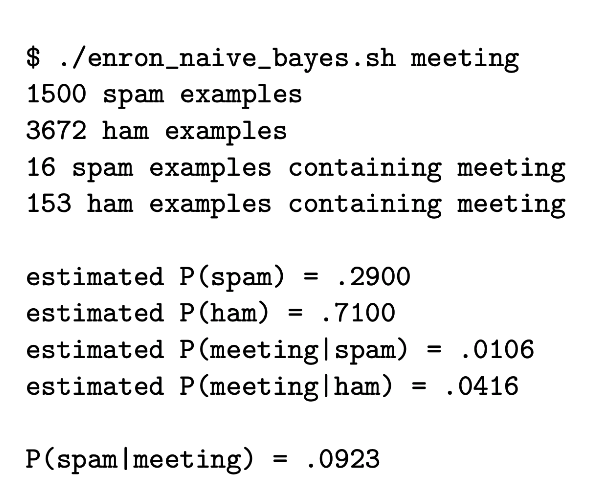
\includegraphics[scale=0.25]{ask2256/figures/enronsh.png}

Let's say we want to know how often the word 'money' appears, we can use grep. We get multiple responses per files, we just want to count the matching files. So we retrieve a list of all the files and the use $\text{wc} - \text{l}$ to count them. 

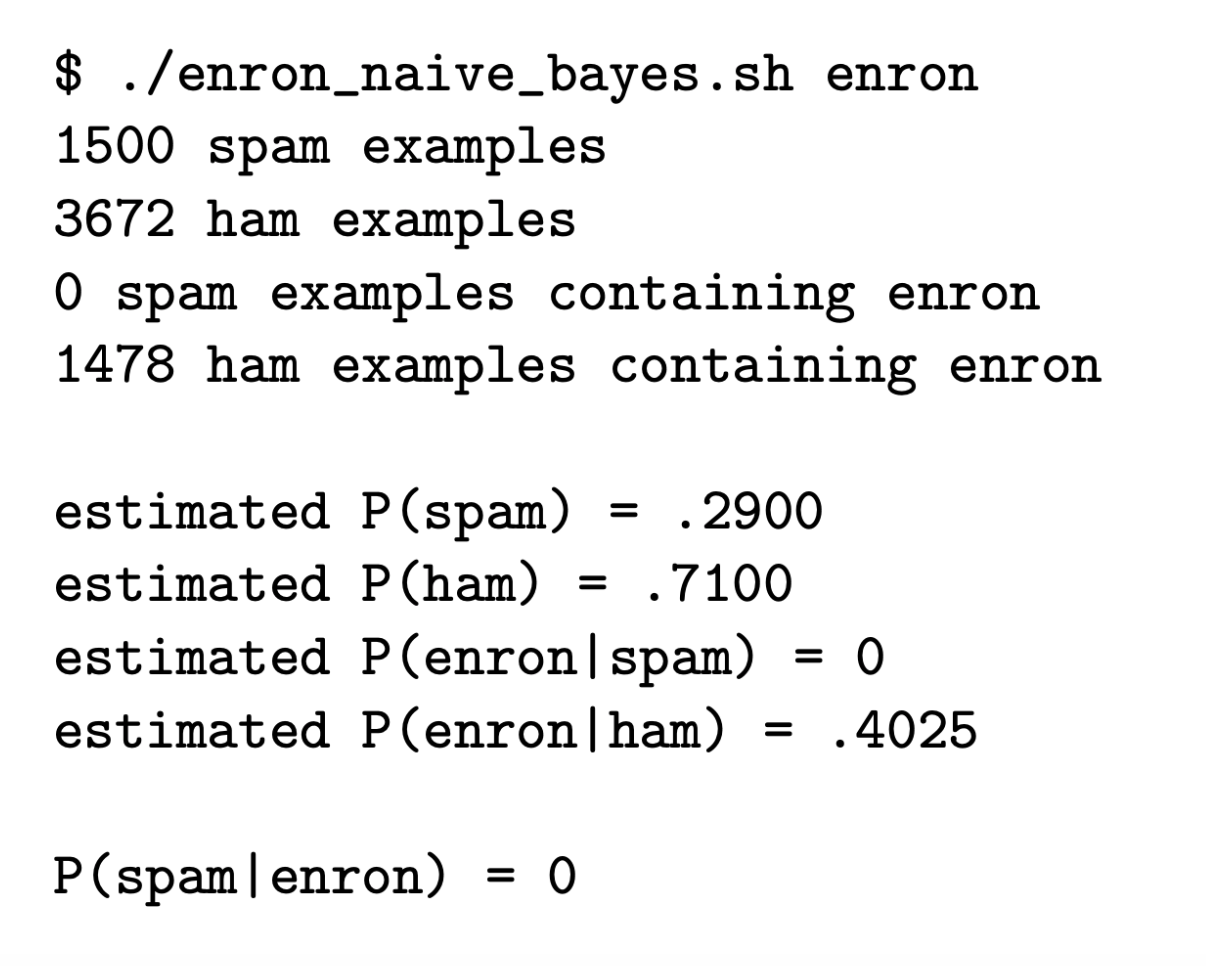
\includegraphics[scale=0.25]{ask2256/figures/enronsh2.png}

Notice that the word ENRON does not appear in the spam classifier. If the spammers just added this word, they would be able to get through. So do we keep it?

We could say $$\hat{p}(w|s) = \frac{n_{w, s} + \alpha}{N_{s} + \beta}$$, where $\alpha = 1$ and $\beta = 1000$.

How do we actually combine this process for a lot of words? That brings us to \textbf{Naive Bayes}. 

\section{Naive Bayes}

We represent each document by a binary vector and each word is independent. That means that if we see the word MONEY, the probability of seeing the word FREE has nothing to do with seeing the word MONEY.

Suppose there are $100,000$ words. We ascribe a 'coin' to them and then flip that coin and record the ones that turn up $1$ or $0$. We can think of it as follows:

$X$ is a big matrix where each row is composed of 1 or 0 to represent if a word occurs or not 

$$X =
\begin{bmatrix}
  0 & 1& \cdots &1 & 0 \\
  1 & 0& \cdots &1 & 1 \\
  \vdots & \vdots & \ddots & \vdots\\
  1 & 1& \cdots &0 & 1 \\
  0 & 1& \cdots &0 & 0 \\
\end{bmatrix}
$$

Now we want to apply \textbf{Bayes' Rule}. Let $\vec{x}$ represent each row, $x_j$ each column. $\theta_c$ represents the probability of observing a document of class $c$. 

$$p(\vec{x}|c) = \Pi_j \theta^{x_jc}_j e^j ( 1- \theta_{jc}^{1-x_jc}.$$

Let us take the $\log$ of both sides so we can solve for $p(\vec{x} | c)$.

$$\log(p(\vec{x})|c) = \sum_j log\bigg[ \theta^{x_jc}_j ( 1 - \theta_{jc})^{1-x_{jc}}\bigg] = \sum_j \Bigg[ x_j \log\theta_{jc} + (1 - x_j) log(1 - \theta_{jc}) \Bigg]$$

\textbf{Aside} Think about why are we adding a million floats if the documents only has 10 words. 

Let's derive the results from the slides:

$$\log(p(\vec{x}|c) = \sum_j \Bigg[ x_j \log\theta_{jc} + (1 - x_j) log(1 - \theta_{jc}) \Bigg]$$

and group like terms together:

$$\log(p(\vex{x}|c) = \sum_j x_j \log\frac{\theta_{jc}}{1 - \theta_{jc}} + \sum_j \log(1 - \theta_{jc}).$$

The first summation represents one term for each non-zero word. The second sum term represents the constant. This is where we get the result seen in the slides. 

Notice,

$$\sum_j x_j w_j + w_o$$

which is just $$\log p ~ \vec{w} \pdot \vec{x} + \text{intercept},$$

where the intercept is just $x_0$. Notice we have just a linear model.

We can eliminate $p(\vec{x})$ by calculating the log-odds, which gives us a linear classifier of the above form:

$$\log\frac{p(1 | \vec{x}}{0 | \vec{x}} = \sum_j x_j \log\frac{\theta_{j1}(1 - \theta_{j0}}{\theta_{j0}(1 - \theta_{j1}} + \sum_j \log\frac{1 - \theta_{j1}}{1 - \theta_{j0}} + \log\frac{\theta_1}{\theta_0},$$

where $w_j = \log\frac{\theta_{j1}(1 - \theta_{j0}}{\theta_{j0}(1 - \theta_{j1}}$ and $w_0 = \sum_j \log\frac{1 - \theta_{j1}}{1 - \theta_{j0}} + \log\frac{\theta_1}{\theta_0}$. This gives us our linear classifier of the form $\vec{w} \dot \vec{x} + w_0$. 

Basically, we are using Bayes rule to get to a linear model. $y=mx+b$ 

We train by counting words and documents within classes to estimate $\theta_{jc}$ and $\theta_c$:

$$\hat{\theta}_{jc} = \frac{n_{jc}}{n_c}$$

$$\hat{\theta} = \frac{n_c}{n},$$

which gives us 

$$\hat{w}_j = \log\frac{\hat{\theta_j}(1 - \hat{\theta}_{j0}}{\hat{\theta}_{j0}(1 - \hat{\theta_{j1}}}$$

$$\hat{w}_0 = \sum_j \log\frac{1 - \hat{\theta}_{j1}}{1 - \hat{\theta}_{j0}} + \log\frac{\hat{\theta}_1}{\hat{\theta}_0}$$

This means we predict by adding the weights of the words that appear int he document to the bias term. 

\textbf{Aside} Idiot's Bayes--Not so stupid after all? (https://pdfs.semanticscholar.org/bd6a/9d35dabbba8132f48835f636cf7c3b3e9c80.pdf)

Training is computationally cheap and scalable, and the model is easy to update given new observations. If we get new data, and we have trained the model based on previous data, we just have to update the counts. Performance varies with document representations corresponding to likelihood models. The big thing is that when we are estimating the $\theta$'s, we have to be careful to cross-validate over the parameters $\alpha$ and $\beta$. 

It is often important to smooth out these parameter estimates to avoid over-fitting as follows:

$$\hat{\theta}_{jc} = \frac{n_{jc} + \alpha}{n_c + \alpha  + \beta}.$$

Going back to log-odds calculations, let us take

$$\log\frac{p(s|\vec{x}}{p(h | \vec{x})}= \vec{w} \dot \vec{x}$$

$$\log \frac{p}{1 - p} = \vec{w} \dot \vec{x}.$$

This is a form of a classifier.

How do we estimate the $w$'s?

$$\frac{p}{1 - p} = e^{\vec{w} \dot \vec{x}}$$

$$p = (1 - p)  e^{w \dot x}$$

$$p(1 + e^{w \dot x}) = e^{w \dot x}$$

$$p = \frac{e^{w \dot x}}{1 + e^{w \dot x}}\frac{e^{-w\dot} x}{e^{-w\dot x}} = \frac{1}{1 + e^{-w\dotx}}.$$

When we plot we get something that looks like this:

INSERT DRAWING

As the function becomes increasingly negative, the likelihood of an email being spam decreases. 

Look at the probabilities of seeing a set of examples $(x_i, y_i)$, where $y_i$ is $\{0, 1\}$.

The product of those probabilities is as follows:

$$L = \Pi_i p^{y_i}_i ( 1 - p_i)^{1 - y_i},$$

where $p_i = p(x_i | \vec{w})$.

so we get

$$\mathcal{L} = \log L = \sum_i \Bigg[ y_i \log p_i + \left(1 - y_i \right)\log(1 - p_i)\Bigg]$$

The best $\vec{w}$ is found as:

$$argmax_{\vec{w}} (p(D | \vec{w}) \log\frac{1}{1 + e^{-w x_i} } = -\log(1 + e^{\vec{w} \dot \vec{x}})$$

Then putting this into our previous statement

$$\mathcal{L} = \sum_j \Bigg[ y_i \log\frac{p_i}{1 - p_i} + \log(1 - p_i)\Bigg],$$

where $\vec{w} \dot x_i = \log\frac{p_i}{1 - p_i}$.

It follows, 

$$\mathcal{L} = y_i ( w \dot x_i ) - \log(1 + e^{w x_i }).$$

Differentiating both sides:

$$\frac{d \mathcal{L}}{d w_j} = \sum_j \Bigg[ y_i x_{ij} - \frac{1}{1 + e^{w  x_i}} e^{w \dot x_i} x_{ij} \Bigg]$$

where $p_i = \frac{1}{1 + e^{w \dot x_i}} e^{w \dot x_i} \pdot x_{ij}$. 

It follows

$$0 = \sum_j (y_i - p_i) x_{ij}$$

We can't invert these matrices because we are not dealing with a linear system. 

This is actually a \textbf{Gradient Descent Method}. We can think of $y_i$ as the actual value and $p_i$ as the predicted, and then scale it by the weight $x_{ij}$.

In the $i^{th}$ document if the $j^{th}$ word appears, and we are wrong we either increase or decrease our prediction. Gradient descent is just guess , check update. too high? lower guess. Too low? higher guess. All of the stuff we had before for linear regression follows through, but we are dealing with non linear prediction, not linear. The purpose is to minimize the error $\epsilon$. We can't minimize this error in stone step (e.g. it's not quadratic), so the surface actually looks quite weird. We are dealing with non-linear Euclidean geometry. 

Why is this different from Naive Bayes? The predictor has the same form. The difference is how we estimate $w_j$. In this case, we are using all the $w_j$'s, then update them to correct the prediction. If things do co=occur, we can learn to share the weight. 

With \textbf{Naive Bayes}, we just count one word. In this one, we are actually, we are taking the derivative with respect to $w$, but it's not separate. When we make the prediction, we are using all the $w$'s. This involves making the prediction, so we are using all the $w$'s and updating. That's how it learns to share between the weights.

\section{Linear Regression Models}

Let us start with some coding. Going back to our model idea, let us think of each row as a word, each column as a probability of being spam or ham?

We can fit a \textbf{Naive Bayes} classifier in R. This gives us the number of words, the class, and what type of character we're dealing with. R contains native Naive Bayes functions, as follows:

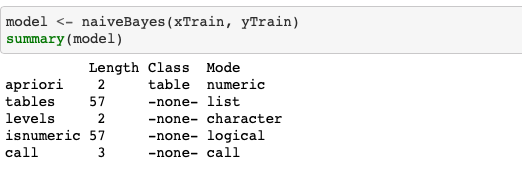
\includegraphics[scale=0.40]{ask2256/figures/naivebayes.png}

Then we construct the confusion matrix. The confusion matrix gives a summary of the classifiers performance, with the actual label determining the row, ad the predicted label giving the column. Here is how we do it in R:

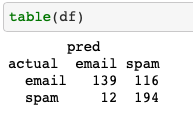
\includegraphics[scale=0.40]{ask2256/figures/confusion.png}

which gives us the following table:

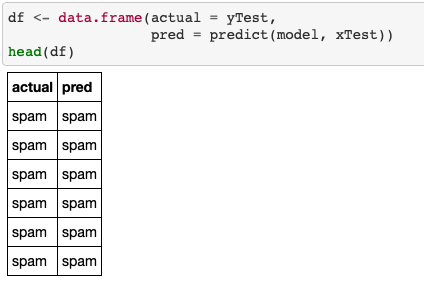
\includegraphics[scale=0.40]{ask2256/figures/confusionmatrix.png}

When we predict and it is spam, we get a \textbf{True Positive}. If something is predicted as spam and actually not spam, this is a \textbf{False Positive} (\textbf{Type I Error}). If something is predicted as not spam and ends up being spam, we get a \textbf{False Negative} (\textbf{Type II Error}). If something is predicted as not spam and ends up not being spam actually, it is a \textbf{True Negative}. This is gives us the concept of \textbf{accuracy}

\textbf{Precision} is the fraction of predicted spam that is actually spam. 

So this would be true positive over true positive plus false positives. Basically, we want true positives over everything that is predicted as being spam. 

We could optimize the $w$'s with precision, but that would be very hard. Instead, we can perform the analysis, then adjust for precision.

Recall: the fraction of all spam that is predicted to be spam is taken as the true positive over false negatives. We are focusing on what was predicted as spam and actually spam over what is predicted as not being spam but ends up being spam. That would be $$\frac{\text{true positive }}{\text{false negative}}.$$ If we want a high recall, then precision increases. 

The false positive rate is the fraction of legitimate email that is predicted to be spam. So we take the false positive (predicted as spam ends up not being spam) and divide by true negatives. 

There are packages built into R that let us calculate all of these rates. The biggest problem with the Native Bayes classifier is overconfidence. But maybe it's not? Maybe everything in the right curve is actually spam in this plot:

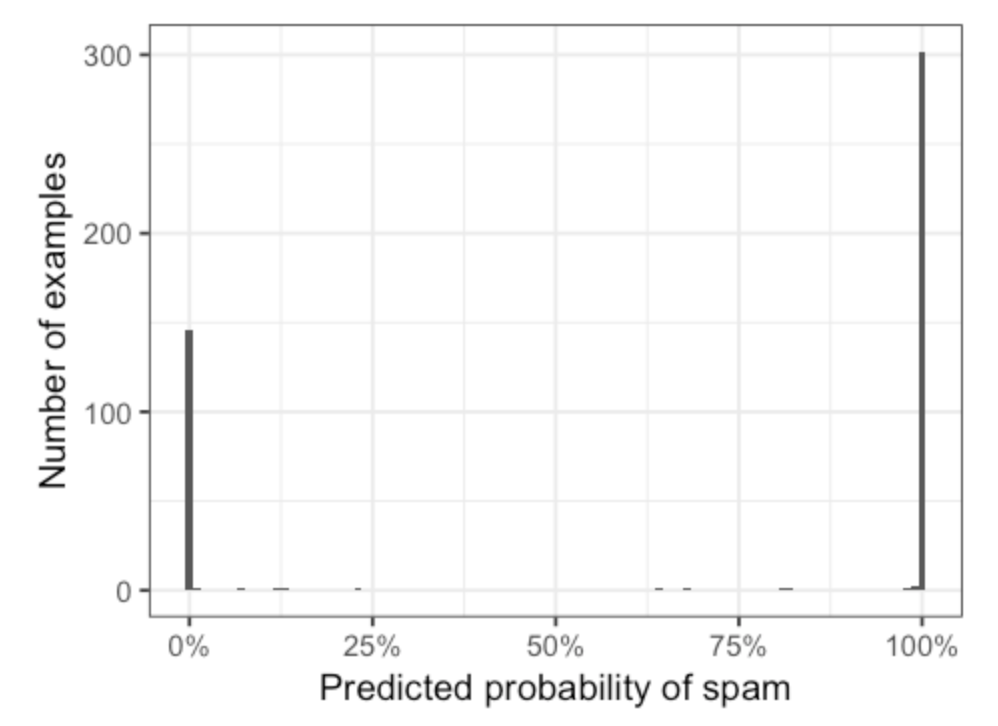
\includegraphics[scale=0.40]{ask2256/figures/overconfident.png}

Let's do this on a fractional basis. Then we get the below plot

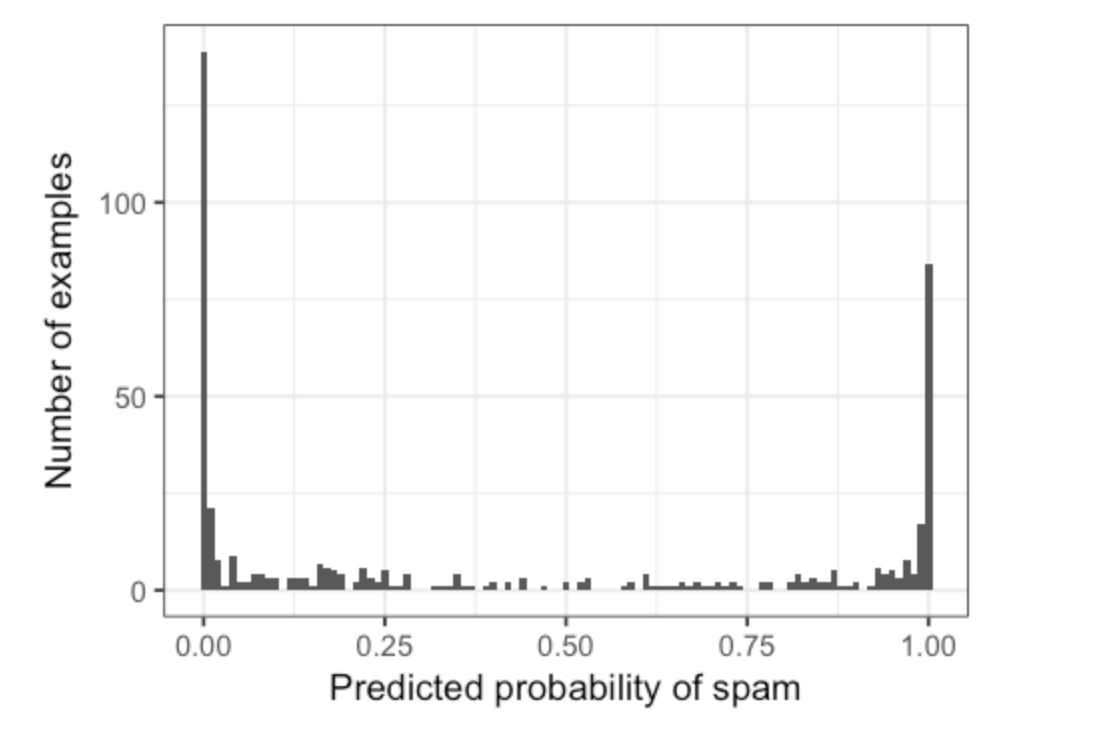
\includegraphics[scale=0.40]{ask2256/figures/fractions_plot.png}

Of the things we were certain were spam, only $75\%$ of them turned out to be spam, of the things that we were certain were not spam, about $5\%$ turned out to not be spam. But this plot does not look very good. 

We can fit a linear regression model by taking the data and saying spam is a function of all the words. We use GLM to do that. We tell it that the outcome is 'binomial' (the $\vec{w} \dot \vec{x}$ corresponds to a coin flip). 

Next, we fit a logistic regression model using the following code. 

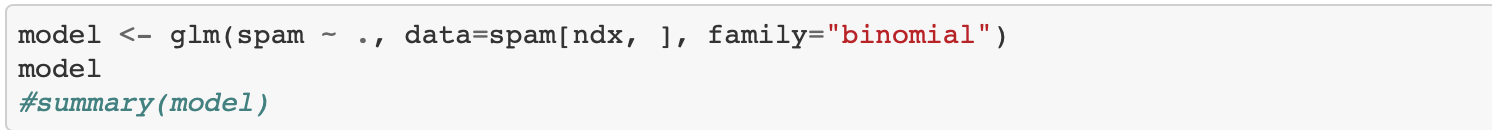
\includegraphics[scale=0.40]{ask2256/figures/glm_code.png}

which yields the following results

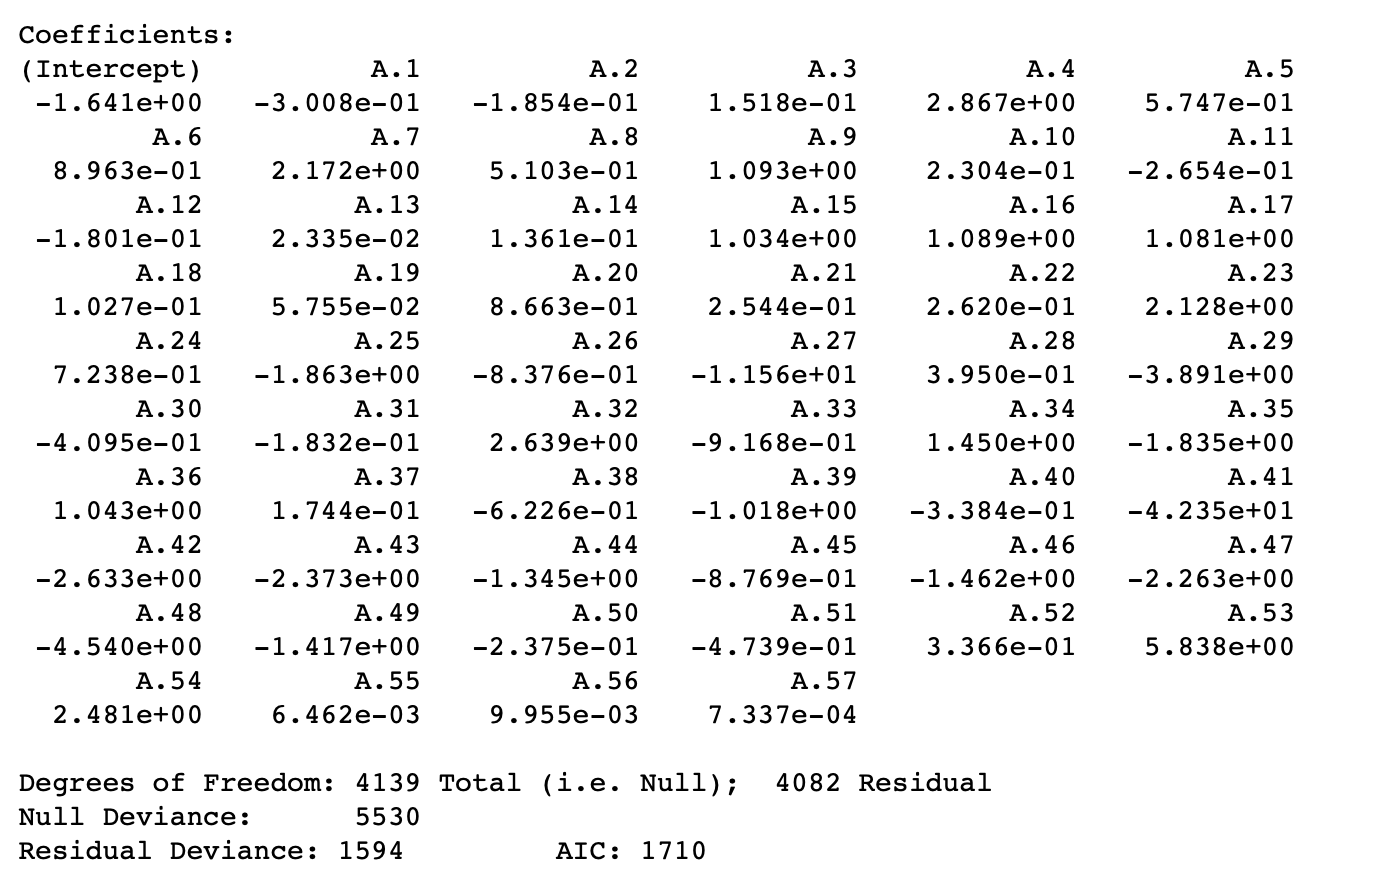
\includegraphics[scale=0.40]{ask2256/figures/glm_results.png}

Coefficients greater than $0$ indicate spam. Coefficients less than $0$ indicate ham. When we compute all the summary stats, we notice that the False Positive Rate has been greatly reduced from approximately $40\%$ to $5\%$! Now $5\%$ of regular emails end up in the spam box. This is much better! 


